\chapter{Løsnings Metoder}	
Der er flere forskellige metoder til at løse et lineært ligningsproblem. 

I dette kapitel vil to forskellige geometriske tilgange til at løse et lineært programmeringsproblem blive gennemgået med udgangs punkt i henholdsvis %indsæt kilder
Den ene gør brug af niveaumængder, mens den anden benytter at basisløsninger kan bruges til at beskrive en simplex.

%Den ene tager udgangspunkt i beviset for Sætning \ref{stn:eksistens}, hvor retnings vektoren vil blive valgt ud fra betragtning af niveaumængden for objektfunktionen. 
%Der vil derfor blive givet en gennemgang af sammenhængen mellem den optimale værdi og niveaumængden med udgangspunkt i %indsæt kilde.

\section{Niveaumængder}
\textbf{Fokus: Sammenskriv, ændre til Niveau mængder og drag paralleller til retningsvektorer}

\begin{defn}
Lad $ \vec{a} \in \mathds{R}^n$, $\vec{a}\neq \vec{0}$ og $b$ være en skalar, da kaldes en mængde for:
\begin{enumerate}
\item En \textbf{Hyperplan} hvis $\{ \vec{x} \in \mathds{R}^n | \vec{a}^{T}\vec{x} = \vec{b}\}$,
\\ \item En \textbf{Halfspace} hvis $\{ \vec{x} \in \mathds{R}^n | \vec{a}^{T} \vec{x} \geq \vec{b}\}$.
\end{enumerate}
\end{defn}


En måde at finde den optimale løsning for lineære programmerings problemer med få variable er ved introduktionen af niveaukurver.
\begin{defn}[Niveaukurver]
Lad $f(\vec{x})= \vec{c}^T\vec{x}$ være en funktion, da er en \textbf{niveaukurve} mængden 
\begin{align*}
N_z = \{\vec{x}| f(\vec{x}) = z, z \in \mathds{R}\}
\end{align*}
\end{defn}
Niveau kurver er dermed den mængde af vektorer, der har samme funktionsværdi for objektfunktionen. 
De vektorer udspænder en linje, som er ortogonal med koefficentvektoren $\vec{c}$.
\begin{stn}[Niveaukurven er ortogonal med $\vec{c}$]
Lad $N_z$ betegne en niveaukurve, til objektfunktionen $f(\vec{x})= \vec{c}^T\vec{x}$, da er $\vec{c}$ ortogonal med linjen udspændt af $N_z$.
\end{stn}
\begin{proof}
Lad $\vec{x}, \vec{y} \in N_z$ da er linjen udspændt af $N_z$ parallel med differensvektoren $\vec{x}-\vec{y}$.
Tages prikproduktet af differensvektoren og vektor $\vec{c}$, fåes at
\begin{align*}
\vec{c}^T(\vec{x}-\vec{y}) = \vec{c}^T\vec{x} -\vec{c}^T\vec{y} = z - z = 0,
\end{align*}
hvorfor at vektor $\vec{c}$ og differencevektoren er ortogonale, og dermed må vektor $\vec{c}$ også være orthogonal med linjen udspændt af $N_z$.
\end{proof}
Den optimale løsning findes så ved at finde det mindste $z$ for hvilken niveaukurven har en ikke-tom skæring med den mulige mængde. 
Hvilket gøres ved at flytte kurven så langt i den modsatte retningen af $\vec{c}$ som muligt.
\begin{stn}[Optimal løsning og -værdi fundet ved niveaukurver]
Lad $f(\vec{x})=\vec{c}^T\vec{x}$ betegne objektfunktionen til et standard minimerings problem med løsningsmængde $\mathcal{F}$, da vil den optimale løsning være givet ved 
\begin{align*}
\vec{x^*}=\underset{k}{\min} \, k \cdot \vec{c} \in \mathcal{F}.
\end{align*}
og den optimale værdi er givet ved
\begin{align*}
z^* = \underset{k}{\min} \, k \cdot \Vert \vec{c} \Vert ^2
\end{align*}
\label{stn:niveau}
\end{stn}
\begin{proof}
Det følger af Sætning %mangler
, at en løsningsvektor $\vec{x}$ kan omskrives til summen af en vektor parallel med $\vec{c}$, kaldet $\vec{x}_p$, og en vektor orthogonal med $\vec{c}$, kaldet $\vec{x}_o$. 
Dermed kan objektfunktionen omskrives til
\begin{align*}
	f(\vec{x}) & \ = \ \vec{c}^T\vec{x}\\
	f(\vec{x_p}+\vec{x_o}) & \ = \ 
	\vec{c}^T\vec{x_p}+\vec{c}^T\vec{x_o} \ = \ 
	\vec{c}^T\vec{x_p} \ = \ 
	k\cdot \vec{c}^T\vec{c} \ = \ 
	k \cdot \Vert \vec{c} \Vert ^2.
\end{align*}
Dermed kan det konkluderes at den optimale løsning er en vektor $\vec{x^*}=\underset{k}{min} k \cdot \vec{c} \in \mathcal{F}$, og den optimale værdi er $z* = \underset{k}{min}k \cdot \Vert \vec{c} \Vert ^2$
\end{proof}
Af Sætning \ref{stn:niveau} følger det også, at den optimale værdi er den vinkelrette afstand fra origo og  linjen udspændt af niveaukurven. 
Det følger af at den optimale værdi er givet, som et multiplum af længden af $\vec{c}$, der står vinkelret på linjen udspændt af niveaukurven.
i
Dette kan ses i  for et maksimerings problem i Eksempel \ref{eks:maksprob3}.


\begin{eks}[Optimal løsning fundet grafisk]
Niveaukurverne $46=\vec{c}^T \vec{x}$ og $25=\vec{c}^T \vec{x}$ er på Figur \ref{fig:maksprob3} indtegnet for programmeringsprogblemet fra Eksempel \ref{eks:maksprob2}.

	\begin{center}	
		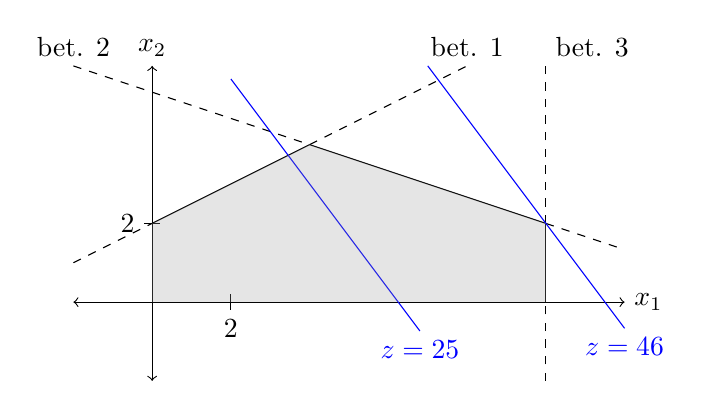
\begin{tikzpicture}
  %laver Grid. godt til når koordinater skal redigeres
  	%\draw[thin,gray!40] (-3,-1) grid (6,3); 
  %x-aksen
  	\draw[<->] (-1,0)--(6,0) node[right]{$x_1$}; 
  %y-aksen
  	\draw[<->] (0,-1)--(0,3) node[above]{$x_2$};
  	
  %akse-markeringer
  	%\node[left] (xakse) at (0,1) {2};
  	\draw[] (-0.1,1) -- (0.1,1) node[pos=0,left] {2};
  	\draw[] (1,-0.1) -- (1,0.1) node[pos=0,below] {2};
  	
  %ligning 1
	\draw[domain=-1:0,variable=\x,dashed] 	plot({\x},{0.5*\x+1});
	\draw[domain=0:2,variable=\x] 			plot({\x},{0.5*\x+1});
	\draw[domain=2:4,variable=\x,dashed] 	plot({\x},{0.5*\x+1}) node[above] {bet. 1};
	
  %ligning 2
  	\draw[domain=-1:2,variable=\x,dashed] 	plot({\x},{-(1/3)*\x+8/3}) node[above] at (-1,3) {bet. 2} ;
	\draw[domain=2:5,variable=\x] 			plot({\x},{-(1/3)*\x+8/3});
	\draw[domain=5:6,variable=\x,dashed] 	plot({\x},{-(1/3)*\x+8/3});
	

  %ligning 3
  	\draw[domain=-1:0,variable=\y,dashed] 	plot({5},{\y});
	\draw[domain=0:1,variable=\y] 			plot({5},{\y});
	\draw[domain=1:3,variable=\y,dashed] 	plot({5},{\y}) node[above right] {bet. 3};
	
  %niveaukurver
  	\draw[domain=3.5:6,variable=\x,blue] plot({\x},{-(4/3)*\x+23/3}) node[below] {$z=46$};
  	\draw[domain=1:3.4,variable=\x,blue] plot({\x},{-(4/3)*\x+25/6}) node[below] {$z=25$};
  	
  %c-vektor
  	%\draw[->,thick,red] (0,0) -- (2,1.5);

  %løsningsmængden skraveret
	\fill[gray!80,nearly transparent] (0,0) -- (0,1) -- (2,2) -- (5,1) --(5,0) --  cycle;
\end{tikzpicture}
		\captionof{figure}{Optimal løsning i den mulige mængde fundet som skæring med ligningen $z=46$.}
		\label{fig:maksprob3}
	\end{center}
	
På figuren ses det, at den største funktionsværdi $z=46$ findes i skæringen mellem bibetingelse 2 og 3.
Ved at løse bibetingelse 2 og 3 som 2 ligninger med 2 ubekendte findes det at den optimale løsning er $\vec{x}=\rvect{10 & 2}^T.$
\label{eks:maksprob3}
\end{eks}

%%%%%%%%%%%%%%%%%%%%%%%%%%%%%%%%%%%%%%%%%%%%%%%%%%%%%%%%%%%%%%%%%%%%%%%%%%%%%%%%%%%%%%
%%%%%%%%%%%%%%%%%%%%%%%%%%%%%%%%%%%%%%%%%%%%%%%%%%%%%%%%%%%%%%%%%%%%%%%%%%%%%%%%%%%%%%

\subsection{Niveaukurver}
Niveaukurver dannes ved fastsættelsen af en funktionsværdi $z=\vec{c}^T \vec{x}$. Niveaukurven er derved mængden af alle vektorer $\vec{x}$, som løser ligningen. Da målet er at maksimere $z$, er målet at finde den største $z$ for hvilken niveaukurven har en ikke-tom skæring med den mulige mængde. 

En løsningsvektor $\vec{x}$ kan omskrives til summen af en vektor parallel med $\vec{c}$, kaldet $\vec{x}_p$, og en vektor orthogonal med $\vec{c}$, kaldet $\vec{x}_o$. Her gælder det derved at, $\vec{x}_p=k\cdot \vec{c}$ for en skalar $k$, og at $\vec{x}_o^T \vec{c}=0$. Dette er muligt, da vektorrummet der er orthogonalt med $\vec{c}$ har dimension $n-1$, mens rummet dannet af $\vec{c}$ har dimension $1$. Da vil vektorrummet dannet af summen af disse rum have dimension $n$, da de to rum er orthononale. Derved kan alle løsningsvektorer $\vec{x}$ udtrykkes som summen af en vektor fra hvert af de to rum.

\begin{align*}
	f(\vec{x}) & \ = \ \vec{c}^T\vec{x}\\
	f(\vec{x_p}+\vec{x_o}) & \ = \ 
	\vec{c}^T\vec{x_p}+\vec{c}^T\vec{x_o} \ = \ 
	\vec{c}^T\vec{x_p} \ = \ 
	k\cdot \vec{c}^T\vec{c} \ = \ 
	k \cdot \Vert \vec{c} \Vert ^2
\end{align*}
Da funktionsværdien derved er lig $k \cdot \Vert \vec{c} \Vert ^2$ gælder det derved om at maksimere $k$ for maksimeringsproblemer og at minimere $k$ for minimeringsproblemer. 


Dette kan ses i Eksempel \ref{eks:maksprob3}.
\begin{comment}
Bør niveaukurve defineres????? Hvordan kan dette bruges, for at finde $z$ er egentlig bare en omskrivning, så der mangler noget argumentation for at $z$ bliver større jo længere væk fra origo man er, hvilket giver ret god mening, men er svært at argumentere for uden at starte på geometri, så måske hele dette afsnit skulle flyttes, måske skal alt om løsninger skal flyttes til geometri?
\end{comment}


\begin{eks}[Optimal løsning fundet grafisk]
Niveaukurverne $46=\vec{c}^T \vec{x}$ og $25=\vec{c}^T \vec{x}$ er på Figur \ref{fig:maksprob3} indtegnet for programmeringsprogblemet fra Eksempel \ref{eks:maksprob2}.

	\begin{center}	
		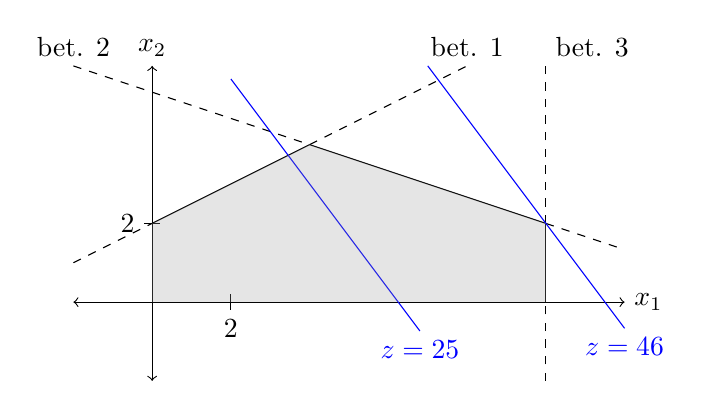
\begin{tikzpicture}
  %laver Grid. godt til når koordinater skal redigeres
  	%\draw[thin,gray!40] (-3,-1) grid (6,3); 
  %x-aksen
  	\draw[<->] (-1,0)--(6,0) node[right]{$x_1$}; 
  %y-aksen
  	\draw[<->] (0,-1)--(0,3) node[above]{$x_2$};
  	
  %akse-markeringer
  	%\node[left] (xakse) at (0,1) {2};
  	\draw[] (-0.1,1) -- (0.1,1) node[pos=0,left] {2};
  	\draw[] (1,-0.1) -- (1,0.1) node[pos=0,below] {2};
  	
  %ligning 1
	\draw[domain=-1:0,variable=\x,dashed] 	plot({\x},{0.5*\x+1});
	\draw[domain=0:2,variable=\x] 			plot({\x},{0.5*\x+1});
	\draw[domain=2:4,variable=\x,dashed] 	plot({\x},{0.5*\x+1}) node[above] {bet. 1};
	
  %ligning 2
  	\draw[domain=-1:2,variable=\x,dashed] 	plot({\x},{-(1/3)*\x+8/3}) node[above] at (-1,3) {bet. 2} ;
	\draw[domain=2:5,variable=\x] 			plot({\x},{-(1/3)*\x+8/3});
	\draw[domain=5:6,variable=\x,dashed] 	plot({\x},{-(1/3)*\x+8/3});
	

  %ligning 3
  	\draw[domain=-1:0,variable=\y,dashed] 	plot({5},{\y});
	\draw[domain=0:1,variable=\y] 			plot({5},{\y});
	\draw[domain=1:3,variable=\y,dashed] 	plot({5},{\y}) node[above right] {bet. 3};
	
  %niveaukurver
  	\draw[domain=3.5:6,variable=\x,blue] plot({\x},{-(4/3)*\x+23/3}) node[below] {$z=46$};
  	\draw[domain=1:3.4,variable=\x,blue] plot({\x},{-(4/3)*\x+25/6}) node[below] {$z=25$};
  	
  %c-vektor
  	%\draw[->,thick,red] (0,0) -- (2,1.5);

  %løsningsmængden skraveret
	\fill[gray!80,nearly transparent] (0,0) -- (0,1) -- (2,2) -- (5,1) --(5,0) --  cycle;
\end{tikzpicture}
		\captionof{figure}{Optimal løsning i den mulige mængde fundet som skæring med ligningen $z=46$.}
		\label{fig:maksprob3}
	\end{center}
	
På figuren ses det, at den største funktionsværdi $z=46$ findes i skæringen mellem bibetingelse 2 og 3.
Ved at løse bibetingelse 2 og 3 som 2 ligninger med 2 ubekendte findes det at den optimale løsning er $\vec{x}=\rvect{10 & 2}^T.$
\label{eks:maksprob3}
\end{eks}


\section{Simplex og Basisløsninger}
Den anden løsningsmetode tager udgangspunkt i resultatet fra Sætning \ref{stn:eksistens}, der siger at en \textbf{optimal løsning ?!?} altid er en basisløsning, og viser hvordan simplexer kan bruges til at vælge en basis, som vil føre til en basisløsning med optimal værdi.
Derfor vil definitionen for en simplex, og hvordan det kan bruges til at udtrykke en basisløsning blive gennemgået i dette afsnit.
\subsection{Simplex}
For at kunne definere en simplex, er det nødvendigt først at introducere begreberne konvekskombination og konvekshyslser.
\begin{defn}[Konveks kombination]
Lad $\vec{x}^1, ...,\vec{x}^k \in \mathds{R}^n$, og $\lambda_1,..., \lambda_k \geq 0 $ være skalare, som opfylder $\sum_{i=1}^k \lambda_i =1$ da er $\sum_{i=1}^k \lambda_i \vec{x}^1$ en \textbf{konveks kombination}.
\label{def:KonveksKombination}
\end{defn}
En konveks kombination er dermed et særtilfælde af en linear kombination, hvor skalrene summer til $1$.
\begin{defn}[Konveks hylster]
Lad $\vec{x}_1, ...,\vec{x}_k \in \mathds{R}^n$, da er $C_{x} = \{\sum_{i=1}^k \lambda_i \vec{x}_i| \vec{x}_1, ...,\vec{x}_k \in \mathds{R}^n, \sum_{i=1}^k \lambda_i =1\}$ et \textbf{konveks hylster} for vektorene $\vec{x}_1, ...,\vec{x}_k$. 
\label{def:Konvekshuld}
\end{defn}
Mens, at mængden af alle konvekse kombinationer af en given mængde vektorer, kaldes et konvekshylster, og minder derfor om spandet af en mængde vektorer.
Et særtilfælde af konveksehylstre er en simplex.
\begin{defn}[Simplex]
Lad $C_x$ være et konveks huld, af $k+1$ affint lineært uafhængige vektorer, da er $C_x$ en $k$-dimentionel \textbf{Simplex}.
\label{def:simplex}
\end{defn}
%Eftersom det konveksehylster, kun består af konvekse kombinationer, vil det give mening at det udgør en konveks mængde.
%\begin{stn}
%Konveks huldet $C_x = \{\sum_{i=1}^k \lambda_i \vec{x}_1| \vec{x}_1, ...,\vec{x}_k \in \mathds{R}^n, \sum_{i=1}^k \lambda_i =1\}$ over en endelig mængde vektorer, er en konveks mængde
%\end{stn}
%\begin{proof}
%Lad $\vec{z}, \vec{y}\in C_x = \{\sum_{i=1}^k \lambda_i \vec{x}_i| \vec{x}_1, ...,\vec{x}_k \in \mathds{R}^n, \sum_{i=1}^k \lambda_i =1\}$ være vilkårlige vektorer da må $\vec{z}= \sum_{i=1}^k \gamma_i \vec{x}_i, \vec{y}= \sum_{i=1}^k \eta_i \vec{x}_i$ for $\sum_{i=1}^k \gamma_i = 1$ og  $\sum_{i=1}^k \eta_i = 1$. 
%Derfor må
%\begin{align*}
%	\lambda \vec{z} + (1- \lambda) \vec{y} &= \lambda\sum_{i=1}^k \gamma_i \vec{x}_i + (1-\lambda)\sum_{i=1}^k \eta_i \vec{x}_i
%	\\ &=\sum_{i=1}^k (\lambda \gamma_i+(1-\lambda)\eta_i )\vec{x}_i,
%\end{align*}
%For $\lambda \in [0,1]$.
%Betragt nu konstanterne 
%\begin{align*}
%	\sum_{i=1}^k (\lambda \gamma_i+(1-\lambda)\eta_i ) &= \lambda \sum_{i=1}^k \gamma_i + (1 - \lambda) \sum_{i=1}^k \eta_i 
%	\\ &= \lambda \cdot 1 + (1 - \lambda) \cdot 1 = 1
%\end{align*}
%Hvorfor at $\lambda \vec{z} + (1- \lambda) \vec{y} $ er en konveks kombination af vektorene $\vec{x}_1, ...,\vec{x}_k $, ifølge Definition \ref{def:KonveksKombination}. 
%Derfor må $ \lambda \vec{z} + (1- \lambda) \vec{y} \in C_x$, hvorfor at $C_x$ er konveks ifølge Definition \ref{def:Konveks}.
%Og sætningen er bevist.
%\end{proof}
%Dermed er en simplex en konveks mængde udspændt af affint lineære vektorer.
%Dette kan bruges til geometrisk at repræsenterer basisløsninger og deres basis matrix.
Simplexer kan da bruges til at repræcenterer en basisløsning.

\subsection{Simplex og Basisløsninger}
For at en basisløsning kan blive repræsenteret af en simplex, kræver det, at basisløsningen er en løsning til et lineært programmerings problem på konveks form.
\begin{defn}[Konveks form]
Et lineært programmeringsproblem på formen:
\begin{center}
\begin{tabular}{l	>{$}l<{$}}
Minimer			& \vec{c}^T\vec{x} \\
med hensyn til 	& A\vec{x} = \vec{b}\\
og				& \vec{e}^T\vec{x} = 1\\
og 				& \vec{x} \geq \vec{0}, 
\end{tabular}
\end{center}
for $\vec{e} =\rvect{1 & \cdots & 1 }^T$,  siges at være på \textbf{konveks form}, og bibetingelsen $\vec{e}^T\vec{x} = 1$ kaldes \textbf{konveksbibetingelsen}.
\end{defn}
Grunden til at $\vec{e}^T\vec{x}=1$ kaldes konveksbibetingelsen, er fordi den sørger for at $\vec{b}$ er en konvekskombination af søjlerne i matricen $A$.
\begin{stn}[Konveks form]
Et hvert lineært programmeringsproblem med $ \vec{0} \notin P$ kan omskrives til konveks form.
\end{stn}
\begin{proof}
I Kapitel \ref{Afsnit:LinProg}
er det gennemgået hvordan alle lineært programmerings problemer kan skrives på standard form med ligheder, derfor er det kun nødvendigt at vise at et hvert lineært programmerings problem på standard form med ligheder kan omskrives til konveks form.
\\ Lad derfor $\vec{x} \neq \vec{0}$ være en løsning til et lineært programmerings problem på standard form med ligheder, da vil 
\begin{align*}
\vec{e}^T \vec{x} = \lambda,
\end{align*}
hvor $\lambda$ er en positiv skalar.
Da vil 
\begin{align*}
\vec{e}^T\vec{x}' = \vec{e}^T\frac{1}{\lambda}\vec{x} = 1.
\end{align*}
For at sørge for at den konvekse form har samme løsningsmængde som det lineære programmerings problem på standard form med ligheder, multipliceres $A$ med $\lambda$, hvorefter at
\begin{align*}
A' \vec{x}' = \lambda A \frac{1}{\lambda} \vec{x} = A \vec{x} = \vec{b}.
\end{align*}
Derfor må et hvert lineært programmeringsproblem med $\vec{b}\neq \vec{0}$ kan omskrives til konveks form.
\end{proof}
Så længe at nulvektoren ikke er en løsning kan ethvert lineært programmerings problem derfor omskrives til konveks form.
Grunden til, nulvektoren ikke må være en løsning er, at prikproduktet af en vilkårlig vektor og nulvektoren vil altid give nul, hvorfor konveksbibetingelsen ikke kan overholdes.
Dermed vil en basisløsning til stort set hvilket som helst lineært programmerings problem, kunne repræsenteres ved en simplex.
\begin{stn}
Lad $\vec{x}$ være en basisløsning til et lineært problem på konveks form, med basismatrix $B$, da vil
\begin{align*}
S_x = \{\vec{v} \in \mathds{R}^{m+2} \mid \vec{v} = \sum_{i=1}^{m+1} \lambda_i \rvect{\vec{B}_i & c_i}^T, \sum_{i=1}^{m+1} \lambda = 1\}
\end{align*}
være en simplex, og $\vec{b}_x = \rvect{\vec{b}& z_x}^T \in S_x$.
\end{stn}
Bemærk at da problemet er på konveks form vil $|I_B| = m+1$ hvis $A$ er en $n\times m$ matrix, da det i følge Sætning \ref{stn:PQ}
kan antages at alle rækker er lineært uafhængige med $\vec{e}$.
\begin{proof}
For at $\rvect{\vec{A}_i & c_i}^T$ for $i \in I_B$ udspænder en simplex, skal vektorene være affint lineært uafhængige.
Derfor vises først at $\rvect{\vec{A}_i & c_i}^T$ for $i \in I_B$ er affint lineært uafhængige.
Antag for modstrid, at de ikke er, da vil der eksistere skalare forskelligt fra $0$ så
\begin{align*}
\sum_{i = 1}^{m} \lambda_i (\vec{A}_{B(i)} - \vec{A}_{B(m+1)} =  \vec{0} \qquad \wedge \qquad \sum_{i=1}^{m} \lambda_i (c_i - c_{m+1})= 0.
\end{align*}
Betragt nu kun $\sum_{i = 1}^{m} \lambda_i (\vec{A}_{B(i)} - \vec{A}_{B(m+1)} =  \vec{0}$, det medføre, at
\begin{align*}
\sum_{i = 1}^{m} \lambda'_i \vec{A}_{B(i)} = \vec{A}_{B(m+1)},
\end{align*}
hvor $\lambda'_i = \lambda_i/(\sum_{i=1}^m \lambda_i)$.
Derfor følger det, hvis de ikke er affint lineært uafhængige, så er $\vec{A}_{B(m+1)}$ en linear kombination af $\vec{A}_{B(i)}$ for $i  \in i,..., m$.
Det strider mod, at $\vec{x}$ er en basisløsning, og søjlerne $\vec{A}_i$ svare til basis variablene for $i \in I_B$, derfor må vektorerne være affint lineært uafhængige. 
Dermed udgør alle konveksekombinationer af $B_i$ for $i \in I_B$ en simplex, $S_x$.
\\ Så vises det, at $\vec{b} \in S_x$. 
Det følger af Definition \ref{def:simplex},
at $\vec{b}_x\in S_x$, hvis der eksistere skalare, der opfylder $\sum_{i=1}^{m+1} \lambda_i = 1$, så $\sum_{i=1}^{m+1}\lambda_i B_{B(i)}  = \vec{b}_x$.
Da $\vec{x}$ er en basisløsning, følger det, at $B \vec{x}_B = \vec{b}_x$ og da $\vec{x}$ er betinget af konveksbetingelsen og $x_i = 0 $ for $i \notin I_B$, må $\sum_{i=1}^{m+1} x_{B(i)} = 1$, hvorfor det følger, at $\vec{b}_x \in S_x$.
\end{proof}
Bemærk at beviset kun inddirekte beviser at søjlerne i en basismarix udspænder en simplex, det kan konkluderes da $B_i$ kun er affint lineær uafhængige fordi $A_{B(i)}$ er, derfor må de også udspænde en simplex, hvor $\vec{b}$ er et element.
\begin{defn}[Simplex forbundet med basisløsning]
Lad $\vec{x}$ være en basisløsning så $x_i = 0$ hvis $i \notin I_B$, da er $S_x$ \textbf{simplexen forbundet med basisløsning $\vec{x}$}, hvis simplexen er lig konvekshuldet udspændt af søjlerne af $\rvect{\vec{A}_i & c_i}^T$ for $i \in I_B$.
\end{defn}
Grunden til at vektorene udvides, er illustreret på Figur \ref{fig:simplex}. 
\begin{center}
	\begin{tikzpicture}
  %x-aksen
  	\draw[->] (-1,0)--(6,0) node[right]{$x$}; 
  %y-aksen
  	\draw[->] (0,-1)--(0,4.2) node[above]{$z$};
  	
  	
%Punkter
    \node[] (A) at (0.5,0.3) {$A$};
    \node[] (B) at (5, 3.5) {$B$};
    \node[] (C) at (3.5, 4) {$C$};
    \node[] (D) at (1, 2) {$D$};
    \node[] (b) at ( 2.5, 0) {$b$};
    
%Simplexer
    \path[thick, color=blue] (A) edge (B);
    \path[thick, color=blue] (D) edge (B);
    \path[thick, color=blue] (D) edge (C);

% Z
 	\draw[domain=0:4,variable=\y, thick, color = orange] 	plot({2.5},{\y});   
  	
\end{tikzpicture}
	\captionof{figure}{ 
	%Hvis de udvidet vektorer antages at være punkter; $A$, $B$, $C$, $D$, da vil koordinaterne svarende til indgangende i søjlerne i basismatrixen ligger i samme $m+1$ dimentionelle rum, mens at punkterne svarende til koefficienterne i objektfunktionen ligge i den $m+2$ dimension. Derfor vil objektfunktions værdi, anses som $\rvect{ \vec{b} & z }^T$, den orange linje, anses som skæringen mellem simplexerne, de blå linjer. 
	}
	\label{fig:simplex}
\end{center}
Det kan bruges til at finde den optimale basisløsning. 
%Grunden til at vektorene udvides, er fordi de udvidet vektorer, antages at være punkter i stedet, da vil koordinaterne svarende til indgangende i søjlerne i basismatrixen ligger i samme $m+1$ dimentionelle rum, mens at punkterne svarende til koefficienterne i objektfunktionen ligge i den $m+2$ dimension.  
%Derfor vil ændringen i værdien for objektfunktionen for to basisløsninger kunne ses som afstanden mellem de to simplexer forbundet med basisløsningerne i den $m+2$ dimension.
\begin{prop}
Afstanden mellem to simplex $S_x$ og $S_y$ forbundet med basisløsningerne $\vec{x}$ og $\vec{y}$ er $|z_x - z_y|$.
\end{prop}
\begin{proof}
For at vise proportionen findes længden af $\rvect{B_x & \vec{c}_B}^T \vec{x} - \rvect{B_y & \vec{c}_y}^T \vec{y}$
\begin{align*}
 \Vert \rvect{B_x & \vec{c}_B}^T \vec{x} - \rvect{B_y & \vec{c}_y}^T \vec{y} \Vert & =  \Vert \rvect{\vec{b} & z_x}^T  - \rvect{\vec{b} & z_y}^T  \Vert
 \\ & = \Vert \rvect{0 & z_x - z_y}^T \Vert = |z_x - z_y|.
\end{align*}
Dermed kan det konkluderes, at afstanden mellem to simplex $S_x$ og $S_y$ forbundet med basisløsningerne $\vec{x}$ og $\vec{y}$ er $|z_x - z_y|$.
\end{proof}
Det betyder, hvis objektfunktionen skal minimeres, skal simplexen, der ligger tættes på $z = 0$, findes, hvorfor der altid skal vælges en simplex, der ligger lavere end den forrige, dvs. en simpelex, hvor en ny basisvariable har en lavere koefficient $c_i$ end den gamle basisværdi.
Det er det simplexmetoden tager udgangspunkt i.



